\part{Partie informatique, électronique}

L'enjeu de cette partie est grand : il s'agit d'une part de détecter la balle, sa position ainsi que les composantes de son mouvement : vitesses de rotation et vitesses de translation. Le système devant pouvoir être utilisé pour tout type de joueurs, on peut estimer que le pire des scénarios est celui d'un jeu d'échange de grand joueur où la balle se déplace en moyenne à 100  km/h ce qui impose de fortes contraintes temporelles pour les parties acquisition et commande. D'autre part, il faut aussi commander le mur pour qu'il se trouve dans la bonne position pour renvoyer la balle où cela a été décidé par l'algorithme de jeu (non étudié ici), ce qui devra prendre en compte de la position du joueur, qu'il faudra donc déterminer.\\

En supposant que la balle est tapée en fond de court et que le mur se trouve sur le fond de court opposé, le système dispose de moins d'une seconde pour faire l'acquisition et déplacer le mur en conséquence. Mais cette hypothèse est peu probable et il y a de grandes chances pour qu'on ne détecte la balle qu'au moment de son passage au-dessus du filet. De plus, le mur se trouvera sur la ligne de service ce qui ne laisse donc au système qu'environ 200ms pour capter la balle et se déplacer en fonction. \\

C'est pour ces raisons qu'un certain nombre de solutions techniques ont du être envisagées aussi bien pour la partie détection de la balle, détection du joueur que déplacement du mur.

\chapter{Détection de la balle}


L'enjeu de cette partie est de détecter la position de la balle ainsi que les composantes de son mouvement : vitesses de translation ainsi que vitesses de rotation. 

Si les premières sont assez faciles à trouver (il suffit de détecter la balle dans deux positions assez proches), les vitesses de rotation se révèlent plus compliquées à obtenir du fait des vitesses de rotation pouvant atteindre 75 tr/s, soit une rotation toutes les 13ms. 

Si on veut détecter cette rotation, dans le cas d'une caméra, il faudrait donc pouvoir au moins acquérir deux images durant cette rotation soit une image toute les 6ms environ. Il a donc été nécessaire de faire un peu d'exploration de différentes techniques d'acquisition afin de trouver la solution la plus adaptée à notre problème.













\section{Détection de la position et de la vitesse de translation}



\subsection{Détection par laser}

\subsubsection{Rideaux de lasers}

Une première méthode pour détecter la position de la balle à différents instants serait d'utiliser des barrières de lasers comme on peut en trouver dans l'industrie pour limiter l'accès à des machines dangeureuses. On peut en voir notamment sur la figure \ref{img_rideaulasers}.

\begin{figure}[h]
\begin{center}
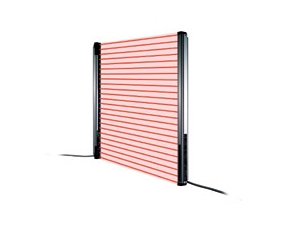
\includegraphics[width=\textwidth]{rideaulaser.png}
\caption{Rideau laser}
\label{img_rideaulasers}
\end{center}
\end{figure}

On a donc besoin d'autant de ces systèmes qu'on veut de positions de la balle (pour la partie calcul et détermination de la trajectoire de la balle), ce qui peut donc vite se révéler très contraignant, tant en termes de coûts que de modularité, mais aussi de positionnement et donc de délai avant impact de la balle avec le mur. En effet, un tel type de procédé peut comporter des risques pour l'utilisateur (utilisation de lasers) et ne peut donc pas pointer vers le joueur. On pourrait donc placer ces capteurs de part et d'autre du filet, mais on limite donc de fait le temps dont on dispose pour déplacer le mur. \\

De plus, il faut un espacement maximal entre deux capteurs lasers de 5cm (une balle de tennis en faisant un peu plus de 6), on a donc besoin d'un nombre de capteurs proportionnel à la hauteur maximale à laquelle on veut détecter le passage de la balle, ce qui aura donc une influence directe sur le prix. Enfin, la plupart des solutions trouvées dans l'industrie ne permettent que de détecter le franchissement (d'objets plus ou moins petits selon l'espacement entre les lasers) et non pas la position où l'objet a traversé le rideau. Il doit néanmoins être possible d'adapter ces solutions, mais cela demanderait du travail supplémentaire. 


\subsubsection{Balayage laser}

\paragraph{Balayage 2D\\}

Une autre solution serait d'utiliser un capteur basé sur un balayage laser. Le principe est quasiment similaire au précédent, c'est-à-dire qu'un balayage 2D nécessiterait d'avoir autant de capteurs qu'on veut de positions de la balle. De la même manière que précédemment, la sécurité de l'utilisateur est aussi à prendre en jeu. \\

On peut donc imaginer un système de capteurs suspendus au plafond, il faut donc prendre en compte la hauteur à laquelle se trouve le capteur pour pouvoir trouver la résolution angulaire minimale à avoir pour pouvoir détecter la balle. À 5m de hauteur, avec un seul capteur pour toute la largeur du terrain, on doit avoir une ouverture angulaire de 94$^{\circ}$, une portée maximale de 7.5m et quelques calculs de trigonométrie donnent une résolution angulaire de minimum 0.25$^{\circ}$. Cependant, à la vue des caractéristiques de différents capteurs de ce type, il ne semble pas que cela soit très contraignant \\ 

La vitesse de la balle va aussi dans ce cas imposer de fortes contraintes sur la fréquence de réalisation des scans. La balle faisant 6cm de diamètre, la taille du faisceau étant d'environ 1cm à la distance citée précédemment, il faut donc que la balle ne parcourt pas plus de 5cm entre deux scans complets, ce qui donne donc une fréquence de balayage de 560Hz. \\

L'ensemble de ces caractéristiques (portée, résolution angulaire et fréquence de scan) semble pour l'instant très dur à trouver (aucune référence chez SICK, et la meilleure référence chez Pulse-In\footnote{http://www.triple-in.de/english/products/2d-laser-scanners/pas/} ne convient pas à nos besoins). 


\paragraph{Balayage 3D\\}

Une solution pour ne pas avoir à multiplier les capteurs est d'utiliser un capteur qui fasse un balayage 3D, ce qui permet donc d'avoir plusieurs positions de la balle avec un seul capteur. Néanmoins, il semble impossible d'avoir un capteur qui puisse avoir une cadence suffisamment élevée pour réaliser ces mesures et le prix d'un tel capteur serait tout simplement beaucoup trop élevé, sachant que la meilleure référence trouvée\footnote{http://www.robotshop.com/eu/fr/capteur-3d-balayage-laser-precision.html} coûte déjà plus de 50 000\texteuro. Malheureusement, même à ce prix, la vitesse de scan est bien trop faible pour pouvoir être utilisée dans le cadre de notre application. 	

\begin{figure}[h]
\begin{center}
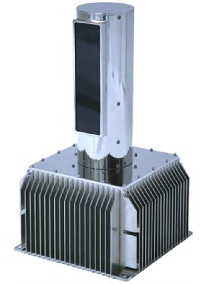
\includegraphics{laserbalyage3d.png}
\caption{Capteur laser à balayage 3D}
\label{img:laser3d}
\end{center}
\end{figure}

\subsubsection{Algorithmie}

La partie algorithmie d'une telle méthode de détection est très simple : le capteur fournit les distances des objets détectés à tous les angles (ou toutes les positions) parcourues par le système. Après avoir réalisé une mesure avec le terrain vide, on note les valeurs obtenues quand il n'y a aucune balle présente, on peut donc ensuite comparer à ces valeurs de référence les nouvelles valeurs et en déduire à quel angle et à quelle distance on a détecté quelque chose. \\ 

Il faut déterminer si le quelque chose est bien la balle et non le joueur (dans le cas où on fait un balayage, sinon on place les rideaux lasers de part et d'autre du filet et il semble évident que le joueur ne va pas jouer au filet contre un mur). Pour ce faire, il suffit de regarder s'il existe plusieurs angles pour lesquels on a détecté quelque chose. Avec une résolution angulaire choisie de manière intélligente, on est sûr que la balle ne puisse pas traverser plus d'un ou deux rayons. On peut donc être sûr dans les autres cas que c'est le joueur qui est détecté.\\ 

Cette solution est donc une solution assez coûteuse et la technologie d'ajourd'hui ne semble pas pouvoir remplir nos besoins en termes de vitesse de détection, de portée et de résolution à la fois. Il s'agit finalement que d'une tâche assez simple et il doit donc exister d'autres solutions qui puissent répondre à nos besoin pour un coût bien moindre. 


\subsection{Détection par caméra}

Une solution alternative à la détection par laser est la détection par caméra. Si cette méthode pose quelques problèmes que l'on a pas avec la détection par laser, elle en résoud certain. On capte en effet une assez grande surface, on n'a donc pas besoin d'une vitesse excessivement élevée pour avoir la balle dans le champ (ce qui est par contre très problématique avec le laser). On a par contre des problèmes de flou que l'on n'avait pas avant. La détection de la balle est aussi plus problématique puisqu'il faut la distinguer du reste de l'environnement qui est visuellement très riche et bourré d'information, dont la très grande majorité est inutile dans notre cas. Bien positionnée, une caméra peut aussi servir à détecter le joueur ce qui est le sujet d'une autre partie. \\ 

Dans le cas où on utilise une caméra, il convient de chosir celle-ci correctement en fonction de notre application. Outre le nombre d'images par secondes, il faut aussi déterminer ses autres caractéristiques : temps d'exposition, sensibilité, type d'objectif... ainsi que son positionnement : au-dessus du terrain ou sur les côtés ? 

\subsubsection{Nombre d'images par seconde et temps d'exposition}

Il convient de rappeler pour cette partie que notre balle se déplace dans le pire des cas à environ 100 km/h, soit environ 28 m/s. Si on ne veut pas avoir de flou de bougé sur la balle, pour l'avoir bien nette, on peut soit augmenter fortement le nombre d'images par seconde, soit définir un temps d'exposition pour la prise des images (ce qui met de fait de côté les caméras grand public puisque diminuer ainsi le temps d'exposition créé un effet saccadé sur le mouvement, ce qui est contraire à la volonté d'avoir des vidéos fluides). La première solution semble quelque peu sous optimale puisque avoir un nombre d'images par seconde élevé (de la centaine à quelques centaines d'images par seconde) est généralement très cher alors que les caméras permettant de régler le temps d'exposition sont beaucoup plus abordables. \\

Avec des caméras rapides, tournant à 60 images par seconde, on a un déplacement entre deux prises de vues d'environ 50 cm, ce qui d'après la simulation, permet d'approximer la trajectoire de la balle à une droite. ce qui empêche d'utiliser une caméra grand public de ce type est que, dans celles-ci, le temps d'exposition correspond à la moitié du temps entre deux images, soit ici 1/120 s, donnant ainsi un déplacement de 25 cm. Avec un tel déplacement, on aura donc une traînée floue assez difficilement exploitable. Cependant, en restant sur une vitesse d'acquisition de 60 images par seconde, si on diminue le temps d'exposition, on peut parvenir à obtenir des images tout à fait nettes. Le flou de bougé existe seulement si l'objet en mouvement parcoure plus d'un pixel sur l'image pendant le temps d'exposition, on choisira donc le temps d'exposition en fonction des caractéristiques suivantes de la caméra. 


\subsubsection{Résolution d'image et angle de vue}





\subsubsection{Algorithmie}

\paragraph{Seuilage sur la teinte\\}

Nous avons donc développé notre algorithme de detection et de calcul de la position de la balle. La première étape était de detecter les pixels correpondant à la balle dans l'image. La balle étant jaune vif nous avons décidé de nous baser sur la teinte pour detecter les pixels en question. La première étape de l'algorithme est donc de convertir l'image définie dans l'espace RGB (Red-Green-Blue : rouge, vert, bleu) vers l'espace HSV (Hue-Saturation-Value : teinte, saturation, valeur). Nous avons constaté que la balle entière avait une teinte comprise entre 80 et 95 (on peut réduire l'écart mais avec le risque qu'une partie de la balle ne soit pas détecté, en contrepartie on récupère moins de bruit). Nous appliquons donc une fonction de seuil qui remplace les pixels dont la teinte est entre nos valeurs limites par un pixel blanc et les autres par un pixel noir.\\

\paragraph{Suppression du bruit\\}

Puis on obtient une image avec la balle de tennis qui apparait en blanc sur une image noire, mais le tout avec beaucoup de bruit comme on peut le voir sur la figure \ref{img_filtragecouleur}. Pour supprimer ce bruit nous avons utilisé des fonctions de morphologie mathématique : érosion et dilatation. L'application d'une dilatation sur une érosion de même élement structurant constitue une ouverture morphologique qui a tendance à eliminer les petits éléments isolés. Ainsi les petits blocs de pixels correspondants au bruits sont éliminés tandis que la balle de tennis qui est un bloc de pixel plus grand que l'élément structurant reste en place. \\ 

Lors de nos tests nous avions beaucoup de bruit à cause notemment de reflets de la balle sur des surfaces brillantes et de nombreuses couleur claires dont la teinte était proches de celle de la balle, nous avons donc opté pour un élément structurant assez gros : un carré de 10 pixels de coté. Il faut donc que la balle soit représentée par plus de 10 pixels pour ne pas être supprimée, ou diminuer la taille de l'élément structurant en supprimant les sources de bruit sur le terrain : pas de vert sur le sol, car proche du jaune en teinte ; pas d'éléments réfléchissant, pas d'éléments jaunes, etc. On comprend aussi l'intéret d'avoir une résolution confortable sur la caméra (FullHd minimum ce qui correspond au minimum à 6 pixels pour la balle au sol, 2500x2000 pixels étant parfait : 12 pixels au sol). Il est à noter qu'il est impossible d'effectuer une érosion ou une dilatation avec un élément structurant plus grand qu'un carré de coté 7. Nous avons donc appliqué deux érosions puis deux dilatations succesives avec un carré de coté 5 comme élément structurant car la composé de 2 érosion/dilatation est une érosion/dilatation avec un élément structurant égal au premier dilaté par le deuxième.\\


\begin{figure}%
\centering
\subfigure[Image originale]{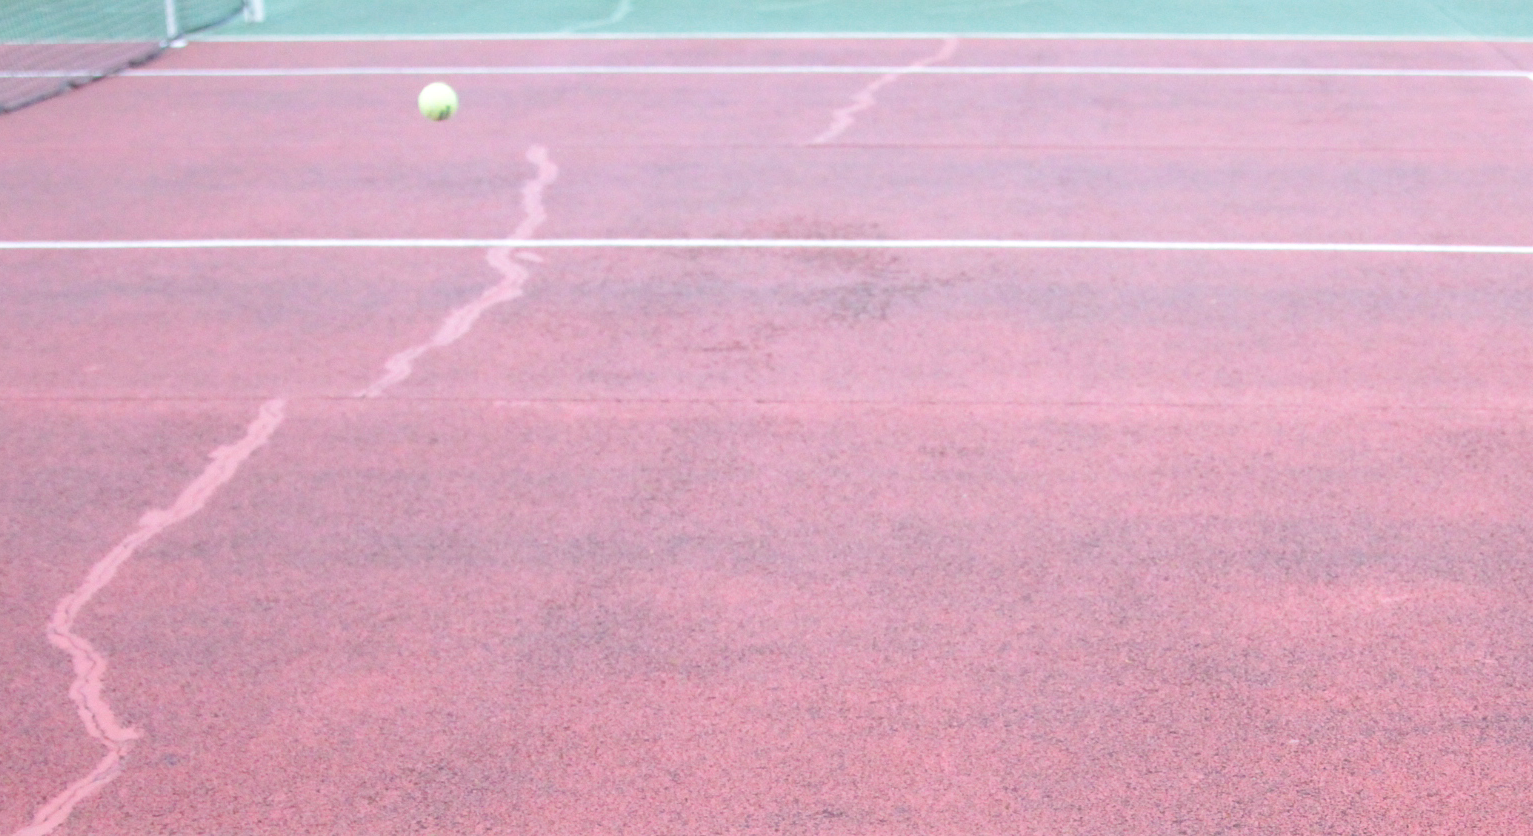
\includegraphics[width=0.45\textwidth]{photo_traitement1.png}}
\subfigure[Image après filtrage couleur]{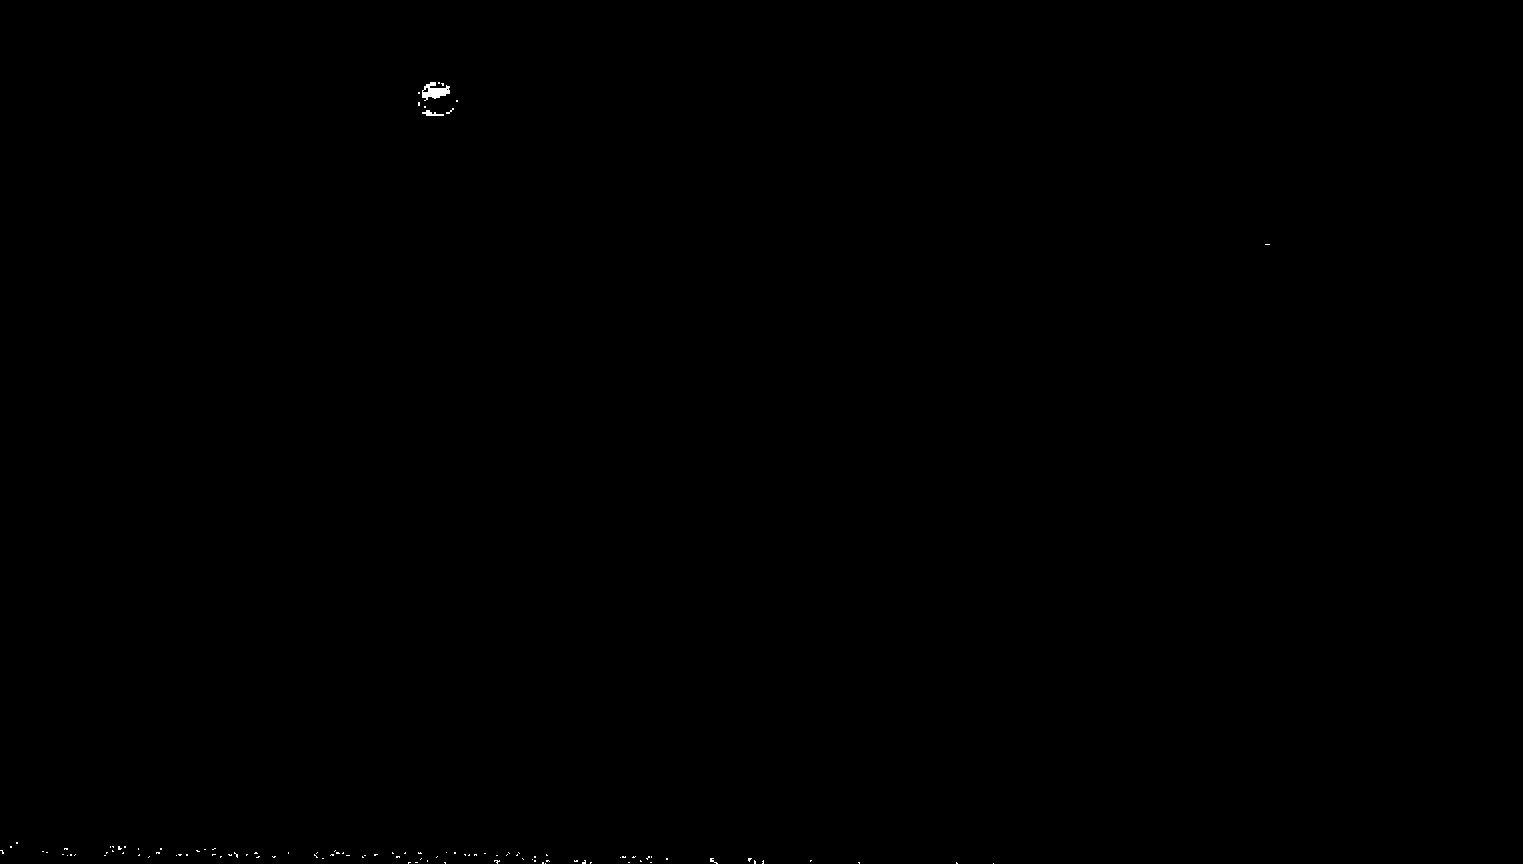
\includegraphics[width=0.45\textwidth]{photo_traitement2.png} \label{img_filtragecouleur}}\\
\subfigure[Image après filtrage du bruit]{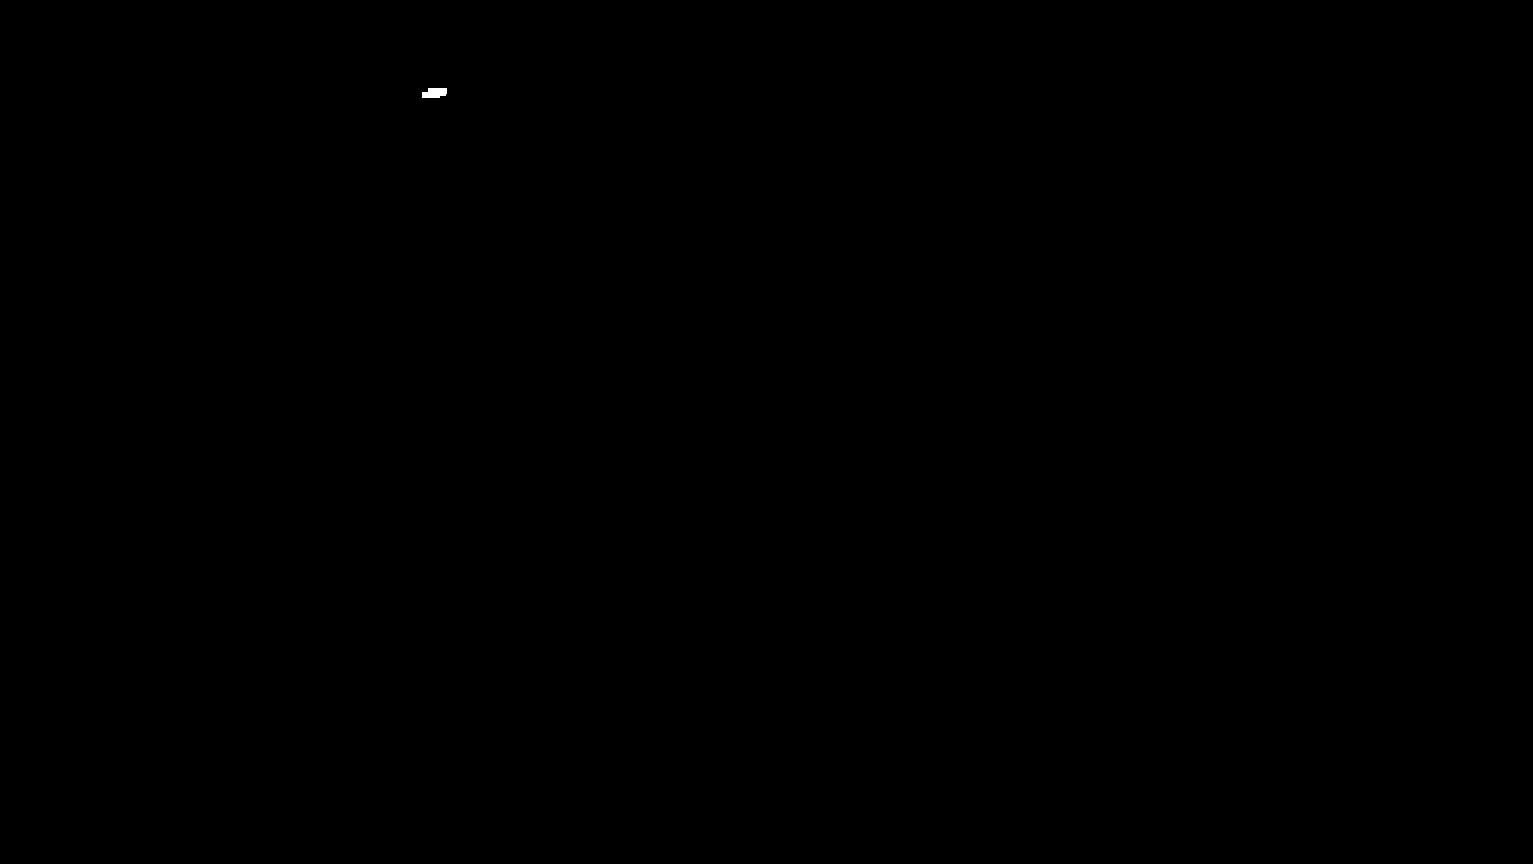
\includegraphics[width=0.45\textwidth]{photo_traitement3.png}}
\subfigure[Cercle détecté à la fin]{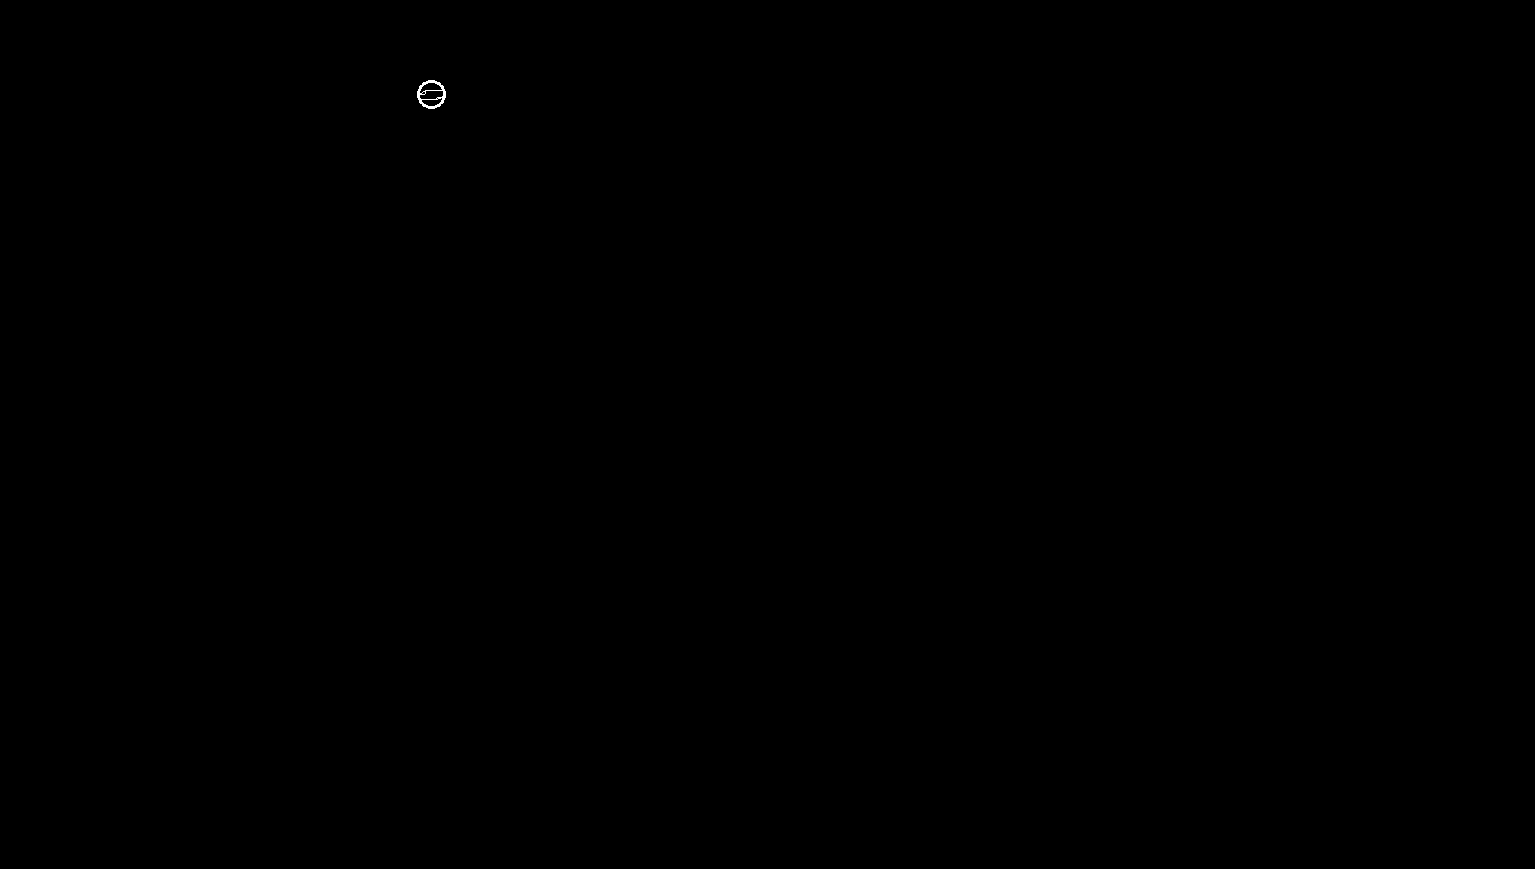
\includegraphics[width=0.45\textwidth]{photo_traitement4.png} \label{3figs-c}}%
\caption{Différentes étapes de la détection de la balle}
\label{3figs}
\end{figure}

\paragraph{Détermination du contour et de la position de la balle\\}

On applique ensuite la fonction findContours de OpenCV, qui permet de trouver les pixels blanc qui forment des blocs et de déterminer les contours de ces blocs. Ensuite il faut déterminer le plus petit cercle englobant ces blocs afin d'obtenir une position en coordonnées de pixel, et un rayon. Pour cela on applique la fonction minEnclosingCircle de la library OpenCV qui nous permet d'avoir le cercle correspondant pour chaque contour. On peut donc récupérer les coordonnées du centre du cercle et son rayon.\\


\paragraph{Détermination de la position de la balle dans le repère lié au terrain de tennis\\}

Grâce à ces informations on peut détecter la position de la balle dans l'espace. Tout d'abord en supposant la caméra en hauteur qui regarde vers le bas, on va chercher à déterminer la profondeur de la balle (axe z, cf figure \ref{img_calculz}). Remarque : les angles ne sont pas orientés.\\

\begin{figure}[h]
\begin{center}
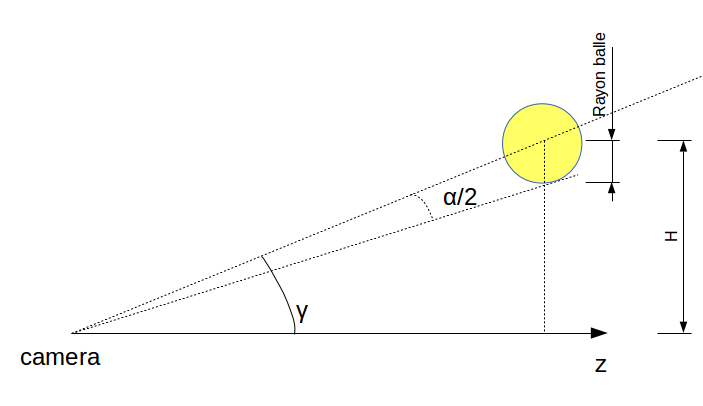
\includegraphics[width=\textwidth]{dessin_calcul_z.png}
\caption{Calcul de Z}
\label{img_calculz}
\end{center}
\end{figure}


$$ \frac{H}{2} = \tan ( \gamma + \frac{\alpha}{2} ) $$
$$ \frac{H - R_{balle}}{z} = \tan \gamma  $$
$$ z = \frac{H - R{balle}}{\tan \gamma} = \frac{z.\tan (\gamma + \frac{\alpha}{2}) - R_{balle}} {\tan \gamma}  $$
$$ z.(1 - \frac{\tan (\gamma + \frac{\alpha}{2})}{\tan \gamma}) = \frac{-R_{balle}}{\tan \gamma} $$
$$ z = \frac{R_{balle}}{\tan (\gamma + \frac{\alpha}{2}) - \tan \gamma}
$$

On trouve $\alpha$ et $\gamma$ de la manière suivante : on a un coefficient Pix2Rad qui dépend de l'angle d'ouverture de l'objectif de la caméra : si on a une longueur en pixel on la multiplie par ce coefficient pour avoir l'angle qu'il y a entre les 2 points représentés par ces pixels, du coup en considérant les coordonnées du point dans l'image en pixels (xPixels, yPixels) avec l'origine au centre de l'image :

$$ \alpha = 2.R_{balle}.Pix2Rad $$ 
$$ \gamma = Pix2Rad.\sqrt{xPixels^2 + yPixels^2} $$

Puis on récupère les coordonnées x et y avec un simple calcul de trigonométrie : on récupère les angles du point selon les axes x et y ($\alpha _x$ et $\alpha _y$) puis :
$$ x = z.\tan \alpha _x $$
$$ y = z.\tan \alpha _y $$


Pour avoir la vitesse il suffit juste de soustraire le nouveau vecteur position par l'ancien et diviser cette quantité par le pas de temps qui sépare la prise de deux images. Pour pouvoir estimer la trajectoire de la balle, il est nécessaire d'avoir trois vecteurs positions et donc deux vecteurs vitesses (explications plus détaillées dans la prochaine partie). 












\section{Détection de la vitesse de rotation}

Un des éléments qui nous paraissait essentiel pour déterminer la trajectoire et le rebond de la balle était la vitesse de rotation de celle ci. En effet il apparait comme trivial qu'une balle qui tourne sur elle même par rapport à un axe parallèle à un plan ne rebondira pas de la même manière qu'une balle sans rotation. Pour le vérifier, il suffit pour celà de se munir d'une balle (de tennis ou autre) de la faire tourner vers soi en la laissant tomber verticalement au sol et la balle va rebondir vers soi.\\

Un autre phénomène rentre en jeu avec des vitesses de rotation relativement élevées, c'est l'effet Magnus. Cet effet découle de la mécanique des fluides. Quand la balle entre en rotation elle déplace des masses d'air et crée des différences de pression autour d'elle même. Ces différences de pression engendre naturellement une pression résultante qui se comporte comme une force. Celle ci peut être verticale et donc porter la balle vers le haut, comme l'est une aile d'avion, ou au contraire vers le bas. Cette effet peut bien sûr faire dévier la balle dans les autres direction suivant les axes de rotations, et on comprend alors tous l'intéret de ces effets qui peuvent dévier la balle d'un mètre dans un sport comme le tennis.\\

La vitesse de rotation maximum qu'un joueur de haut niveau peut fournir est d'environ 100 tours par seconde, ce qui ne pouvait donc pas être mesuré simplement, mais on considére que la vitesse de rotation de la balle est constante durant son trajet durant entre 0.5s et 1s.

\subsection{Caméra ultra-rapide}

Lors de notre première approche, nous nous sommes dit : Puisque la balle tourne très vite, mesurons la à très haute vitesse aussi, ainsi on décomposera aisément son comportement et donc sa vitesse de rotation selon les 3 axes. En nous fixant 100 tours par seconde comme limite, il faudrait voir un même point de la balle passer d'une position à une autre sans passer par la face cachée de la balle entre temps. En admettant que l'on voit bien un bon tiers, voire deux cinquièmes de la balle (les bords de la moitié visible ne sont pas de très bonne qualité et pas facilement exploitables). Nous avons ensuite considéré qu'il faudrait qu'un point ne puisse parcourir que la moitié de cette zone claire pour que l'on détermine la vitesse de rotation sans trop d'ambiguité. Ce qui au final nous fait un cinquième ou un sixième de balle qui défile à 100 tours par seconde entre 2 images, soit une caméra à 500-600 images par secondes minimum.\\

Nous avons donc effectué de nombreuses recherches de caméra de ce type avec une résolution correcte. En effet soit cette caméra sert à détecter la position et vitesse linéaire de la balle comme vu précédemment, soit elle vient se supplanter au système. Dans le premier cas il faut imaginer une caméra qui voit le demi terrain imaginons par dessus : la caméra devra alors être capable de couvrir 11.9 mètres en longueur et des motifs sur la balle. Au début nous avions imaginé traiter les bandes blanches se trouvant sur la balle, faisant 2 mm d'épaisseur en étant généreux. Ce qui nous fait un rapport de 5500 avec la balle au sol, c'est à dire qu'en ayant 5500 pixels de définition dans le sens de la longueur, on pouvait s'assurer d'avoir tout la longueur du demi-court et d'avoir la ligne blanche de la balle présente sur 1 pixel ... Bien sûr c'est en prenant les conditions extrêmes car la balle est rarement au sol mais en l'air ce qui la rapproche de la caméra et la grossit donc, et nous aurions put développer des marqueurs additionnels plus gros, et de couleur sûrement moins difficile à traiter que du blanc alors que le marquage des terrain est en blanc.\\

Cette solution fût vite abandonnée à cause de ce problème de résolution et des surcoûts en terme d'argent et de temps de traitement qu'elle engendrait. Néanmoins l'idée d'une caméra rapide nous semblait toujours être la meilleure solution ne nécessitant pas un matériel trop particulier de la part du tennisman (ou de la tenniswoman !). L'idée était donc de diminuer la résolution nécessaire, donc de cadrer une image moins large. Nous sommes dit qu'au dessus du terrain celà demanderait de mettre la caméra relativement basse et pouvait être dangereux, donc nous avons étudié une camera sur le coté, à la hauteur du poteau du filet. Ainsi elle ne pourrait cadrer par exemple que 3 mètres ce qui ramenerait notre rapport à 1500 ce qui correspond environ à de la full HD, tout à fait abordable. L'inconvénient étant qu'on ne détecte la balle au dernier moment et le mur n'aura donc pas énormément de temps pour se mettre en place. Une idée naïve serait de se dire que l'on peut placer la camera plus loin dans le terrain par exemple à 6m du filet, mais si la joueur doit monter au filet on ne verra plus rien du tout, ce qui est pire que tout.\\

Finalement après moult recherches nous avons trouvé la caméra M3 de IDT qui correspondait assez bien à nos attentes à un prix contenu (15000€ tout de même), puis nous avons trouvé la Edgertronic qui nous paraissait miraculeuse pour son tarif, mais nous sommes vite rendus compte qu'elle ne proposait bizarrement pas de mode streaming, et ne pouvait fournir une vidéo que par carte SD, ce qui était plus que gênant pour notre système temps réel.\\

Mais le véritable problème de cette solution était la vitesse à laquelle il fallait traiter les images (2ms à 500 images par seconde). Nous n'avons pas réalisé d'algorithme pour cette détection de vitesse de rotation, mais il serait à notre goût plus coûteux que la détection des coordonnées x,y,z ;
% Bouger la partie perf dans la partie détection position  %
 et déjà ce dernier nous prenait 70-75ms pour une image au début, ce qui nous a mis un gros coup de doute sur la réalisation de notre idée. Ensuite en essayant sur un ordinateur de bureau récent et puissant nous avons constaté que nous gagnions à peine 5ms par image, mais que OpenCV n'utilisait pas toutes les ressources CPU, uniquement la moitié de la puissance sur place (les 4 coeurs tournaient à 50\% d'après le moniteur système). Nous sommes donc décidés à faire passer les calculs par la carte graphique de cet ordinateur de bureau à travers le module OpenCL de OpenCV (c'est une carte AMD, le module gpu est donc incompatible car écrit en CUDA), ce qui ne fût pas sans difficultés, notamment au niveau des pilotes sous linux. Finalement après quelques jours de configuration le programme s'est mis à tourner sur GPU, et là les gains nous émerveillèrent ! Après application d'une ou 2 fonctions sur gpu le temps passa déjà vers les 50ms. Puis les optimisations diverses ainsi que le portage d'un maximum de fonctions sur GPU nous ont amené à un temps de calcul de 11.5ms par image, en prenant en compte que 3.2ms est due à l'acquisition de l'image à partir du fichier vidéo, à voir si ce temps sera beaucoup plus court avec un système de streaming. Malgré notre bohneur face à cette explosion de performance, le taux de traitement ne plafonne qu'à 85Hz (en FullHD), encore très loin des 500Hz avec un algorithme sûrement plus complexe. Voilà pourquoi nous avons définitivement abandonné l'idée d'une caméra ultra-rapide sur ce projet.


% Parler de la partie filtrage infrarouge dans une partie amélioration de la technique de détection dans la partie détection position, faire un rappel ici %
% PARLER DES CAMERA INFRAROUGE

Malgré tout nous avions imaginé utiliser une imagerie infrarouge pour obtenir directement une image en niveau de gris, où certaines parties de la balle réfléchirait les infrarouges. Ainsi les traitement associés à cette image seraient largement réduit, au niveau du filtrage et de la suppression du bruit. Pour celà nous avions imaginé avoir un éclairage infrarouge qui illumine le demi-court de tennis où est le joueur, et que la balle possède des parties réfléchissante qui ressortiront très clairement sur les images. Pour celà nous avions pensé à coller des bandes réfléchissante sur la balle. Cependant cette solution apparait comme plus que limité car on modifie la surface de rebond de la balle donc sa réaction au sol, et la bande risque de se décoller à tout moment en raison des chocs qui sont appliqués sur cette zone. Nous avions donc imaginé ensuite d'appliquer quelque chose qui réfléchissent les infrarouge et qui adhère fortement à la balle. La zone qui nous paraissait encore la plus propice était la bande blanche parcourant la balle de tennis, car un peu creusée et qu'elle rentre moins en contact lors des rebonds. Et une peinture réfléchissante nous apparut comme une bonne solution car elle peut être appliquée finement sur un contour non droit et adhère relativement bien. De plus les peintures d'isolement utilisées dans le bâtiment sont des des peintures réfléchissantes d'infrarouges.\\

Le problème a encore eu lieu au niveau des caméras : au début nous avons regardé le choix en caméra à infrarouges à haute vitesse. Et le choix était assez limité, en général avec des résolution dérisoires proches du VGA, ce qui était trop peu pour notre traitement. Puis nous nous sommes dit qu'il suffirait de prendre une caméra haute vitesse classique et d'appliquer un filtre infrarouge physique devant son objectif (moins de 100€ pour un bon filtre) et donc que cette caméra ne capterait qu'un peu de rouge au niveau des pixels excités par le rayonnement infrarouge. Le problème est que nombre de caméra ont un niveau de sensibilité réduit au domaine du visible voir à un niveau légèrement plus restreint comme on peut le voir sur le graphe du spectre de réponse de la M3. Les infrarouges qui passerait le filtre n'exciterait donc pas les capteur de la caméra et on obtiendrait alors un image tout simplement noire.\\

Il est à noter qu'un éclairage infrarouge aurait put aussi constituer une gêne pour le joueur, car ce rayonnement l'aurait chauffé comme le fait un radiateur, et que pendant un effort intense, cela peut être très inconfortable.

% INSERER GRAPHE REPONSE SPECTRALE M3

\subsection{Caméra normale}

Ce n'est pas parce que nous avons abandonné l'idée d'une caméra ultra-rapide que nous avons abandonné par la même occasion l'idée d'une caméra. Comme nous l'avons vu précedemment avec la vitesse de notre algorithme, nous avons estimé que nous pourrions traiter sans problème un flux de 60fps. Il est clair qu'à 60 fps, même avec un temps d'exposition réglable, qu'entre 2 images, un marqueur sur la balle aura largement tourné autour de la balle à la vitesse maximum de 100 tours par seconde. L'astuce consiste donc à se dire qu'avec un "long" temps d'exposition, on a des flous, plus précisémment des trainées, et elles peuvent s'avérer très utiles pour connaitre la rotation de la balle. Imaginons que la balle tourne autour d'un axe qui est celui qui vertical dans le plan de la feuille. Imaginons maintenant que l'on met un marqueur facilement détectable en traitement de l'image. La balle va tourner en avancant, Donc pendant le temps d'exposition la balle aura avancé (vers la gauche par exemple) et le marqueur sera passé une ou plusieurs fois devant la caméra, laissant une ou plusieurs traces d'une certaine longueur (voir figure ci dessous).

%INSERER FIGURE EXPLICATIVE

En connaissant la vitesse de la balle et la vitesse de la caméra, on peut en déduire la vitesse de rotation de la balle grâce aux nombre de trainées et à leur longueur. Seulement on a imaginé ici le cas avec une seule composante. En imaginant que la rotation ait aussi une composante selon l'axe de la largueur de la feuille on imagine que les trainées ressembleront à des virgules et que le calcul des vitesses de rotations se complexifie largement. Ajoutons maintenant 2 composantes à notre vitesse de translation, et une troisième composante à la rotation, ce qui représente la réalité. Eh bien on se retrouve avec quelque chose d'indigeste et nous n'avons rien put conclure de ces trainé en multidimensionnel ... Nous avons imaginé mettre des marqueurs parfois exotiques pour avoir des trainées distinctes selon les axes en jeu, mais rien de concluant n'est ressorti de cette étude, et nous avons donc définitivement abandonné l'idée de capter cette information de rotation directement par une(des) caméra(s).\\

Nous avions aussi imaginé la solution infrarouge avec une caméra normale pour obtenir notre trainée, mais les problèmes intrinsèques à ces trainées restaient toujours présent et nous n'avons donc pas put conclure sur quelque chose de satisfaisant.\\

\subsubsection{Algorithmie}


\subsection{Balle intelligente}

Maintenant que notre option caméra était bel et bien enterrée, il nous fallait trouver une autre technologie pour acquérir ces données. Malgré le principe que nous nous étions fixé au départ de ne pas imposer trop de contraintes au joueur (balle spéciale, etc), nous ne voyions pas comment calculer cette vitesse sans données optique en sachant que la balle se déplace "aléatoirement" dans un volume relativement grand. Une solution assez naïve mais pas idiote est de placer le capteur, un gyromètre, directement dans la balle, avec une source d'énergie type pile, un controlleur de base et un module de communication sans fil type bluetooth (moins gourmand et les besoins en débit sont plus que limité : 3 doubles de temps en temps). Ainsi le mur peut interroger régulièrement la système de la balle (4 à 10 fois par seconde par exemple), en prenant en compte que plus on l'interroge, plus la pile se videra vite. On a donc une donnée sur la rotation relativement fiable accessible facilement sans calcul. Evidemment ce système a des inconvénient non négligeables : la balle coûtera sensiblement plus cher qu'une balle classique et ne se trouvera pas dans le décathlon du coin, alors qu'une balle vieillit relativement vite au tennis. Par ailleurs la source d'énergie pourra être amené à s'épuiser plus vite que ne l'est la durée de vie de la balle. Nous avons donc pensé au récent système de recharge sans fil qui pourrait remédier à ce problème. Nous n'avons cependant pas de donnée sur la consommation d'un tel système embarqué pour faire une estimmation de la durée de vie de la pile. Par ailleurs il pourrait être utile de pouvoir éteindre le système, car un module comme le bluetooth, même sans envoyer de données, est relativement énergivore, ce qui pourrait poser problème. Mais nous n'avons pas trouvé d'idée cohérente face à ce problème en prenant en compte que le système est isolé par un couche hermétique. \\

Par ailleurs avec un tel système dans la balle on peut imaginer que son équilibrage peut être altéré de façon plus ou moins importante selon le poids du module embarqué, et que ce déséquilibrage peut entrainer une gène pour le joueur de tennis ainsi qu'une modification du comportement de la balle qui a été étudié dans la partie mathématiques. Enfin il faut trouver un système relativement résistant, pour subir des forces centrifuges extrèmes ainsi que des accélérations hors du commun (quelques centaines de g). Néanmoins, il semble qu'un tel système soit tout à fait réalisable puisqu'Adidas a annoncé la commercialisation de sa Smart Ball pour le mois de Juin 2014. C'est un ballon de foot connecté et bourrée de capteurs qui permet d'analyser les coups et de retranscrireavec une grande précision la trajectoire de la balle (apparemment sous la condition d'une frappe de plus de 10m). 

\begin{figure}[h]
\begin{center}
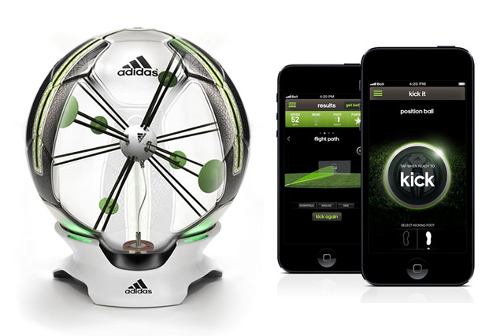
\includegraphics[width=\textwidth]{ballefootintelligente.png}
\caption{Smart Ball d'Adidas}
\label{img:ballefootintelligente}
\end{center}
\end{figure}

\subsubsection{Algorithmie}

Dans ce cas 2 options algorithmique sont possibles : \\
- soit on interroge la balle à temps constant, par exemple 100 ou 200ms (pas trop souvent pour économiser sa batterie, et pas trop peu pour avoir le temps de réagir si la balle a bien avancé depuis la dernière interrogation). Puis à chaque nouvelle donnée on met à jour les données correspondantes sur la partie calcul mathématiques.
- soit on attend d'avoir une vitesse de balle positive (balle qui avance vers le mur) pour faire la requête, ce qui économisera le nombre de requètes, cependant il existe une latence non négligeable (de l'ordre de 100ms) sur tous les systèmes sans fil. Il est donc possible que cette latence ne nous permette pas d'avoir le temps de calculer les données pour le mur

\subsection{Raquette intelligente}

Par hasard en cherchant des solutions sur internet, nous sommes tombés sur un produit intéressant sur le site de Babolat, un fournisseur de matériel de tennis. C'était leur raquette Play and Connect. Cette raquette est bardée de capteur et d'un micro ordinateur dans son manche. Ainsi elle est capable d'analyser nombre d'information sur chaque coup joué par le joueur comme le montre cette page web : https://www.babolatplay.com/features \\

De plus la raquette est équipée d'un module bluetooth qui permet de diffuser ces informations en temps réel, initialement prévu pour envoyer ces données à un smartphone possédant l'application dédiée, mais il est concevable de détourner cette fonction pour récupérer ces données sur le PC du mur. Au niveau des contraintes, comme on peut s'y attendre, le prix de la raquette est deux fois plus élevé qu'une raquette de même qualité sans électronique embarqué et devrait avoisiner les 500€. Une autre contrainte est celle de l'autonomie de la raquette, celle ci étant de 6h selon le constructeur, elle apparait comme très correcte pour un entrainement de tennis, même de longue durée.\\

Cependant le système actuel ne serait pas capable de fournir la vitesse de rotation de la balle. Mais il serait peut-être possible de l'obtenir mathématiquement grâce aux informations de puissance, de spin, etc mais nous n'avons pas eu le temps d'étudier ce modèle. Il est à noter qu'une prochaine version de cette Babolat Play and Connect pourrait fournir ces informations et donc être une solution de choix pour ce mur de tennis intelligent.

\begin{figure}[h]
\begin{center}
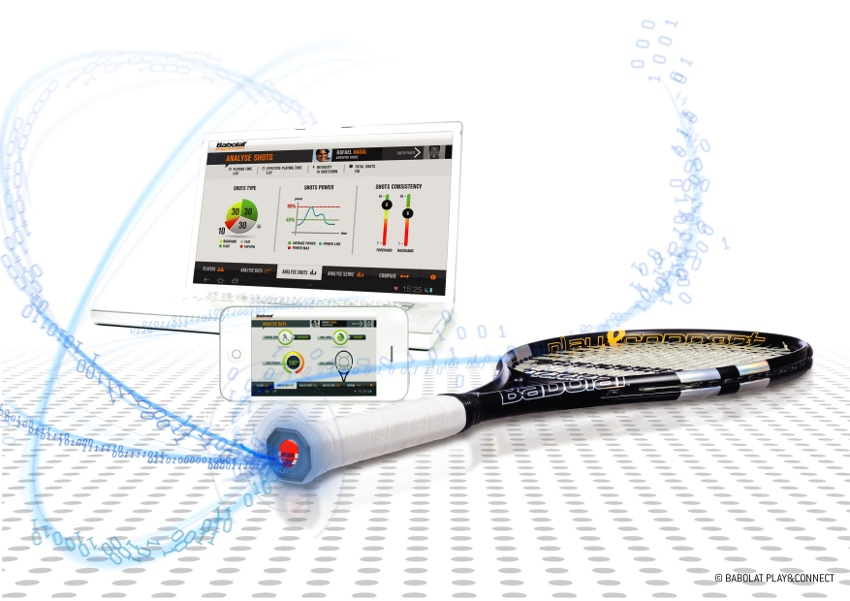
\includegraphics[width=\textwidth]{babolatplayandconnect.jpg}
\caption{Babolat Play and Connect}
\label{img_babolatplayandconnect}
\end{center}
\end{figure}


\subsubsection{Algorithmie}











\section{Conclusion}






















\chapter{Détection du joueur}

On s'intéresse dans cette partie à la détection du joueur, pour pouvoir décider de la position de la balle que l'on renvoie avec le mur en fonction du style de jeu qui aura été décidé par le joueur lui-même. On s'intéressera donc aussi bien à la position du joueur mais aussi à son déplacement, pour pouvoir déterminer son intention (pour pouvoir prendre le joueur à contre-pied par exemple), mais aussi l'effort fourni depuis le début de l'entraînement (nombre de calories brûlées, distance parcourue et autres statistiques du genre). \\

Cette partie est bien moins complexe que la précédente étant donné les vitesses de déplacement bien moindre donc des contraintes temporelles moins fortes et aussi une précision requise bien inférieure à celle requise pour la détection de la balle. Comme dans le cas de celle-ci, on a une multitude de solutions techniques qui permettent de réaliser cette détection. Si certaines solutions pour la détection de la balle permettent aussi de détecter la position du joueur, il peut être bon d'avoir un capteur dédié à cela, les données provenant du capteur détectant la balle peuvent servir à confirmer celles de la solution dédiée.


\section{Balayage laser}

Une des premières approches serait d'utiliser un balayage laser pour détecter le joueur. En fonction du positionnement du capteur, on peut vouloir un balayage sur 90$^\circ$ dans le cas d'un capteur sur l'un des côtés du filet (ou dans un des coins du terrain, côté joueur) , ou 180$^\circ$ si on décide de placer le capteur au centre du terrain au niveau du filet. On préferera placer les capteurs au niveau du filet puisque si on les place côté joueur, il faut laisser une certaine distance de sécurité pour qu'ils ne gênent le joueur dans aucun cas, ce qui fait augmenter la portée que doit avoir le capteur. Dans ce dernier cas, les capteurs sont aussi plus sujets à prendre des coups s'ils sont placés derrière le joueur (balles non rattrapées par le joueur par exemple). La figure \ref{img_joueurpositionlaser} reprend les différentes configurations possibles pour le positionnement du capteur. 

\begin{figure}[h]
\begin{center}
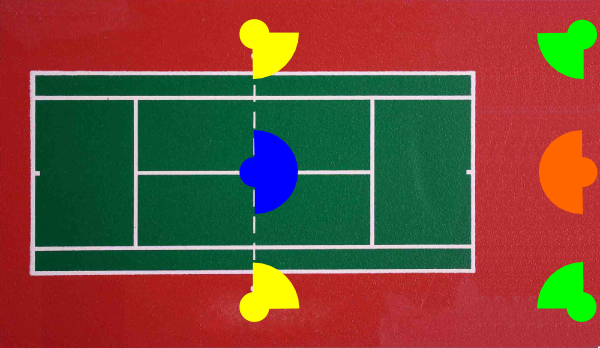
\includegraphics[width=\textwidth]{joueurpositionlaser.png}
\caption{Différents positionnement du capteur à balayage}
\label{img_joueurpositionlaser}
\end{center}
\end{figure}

Comme expliqué dans le chapitre sur la détection de la balle, la partie traitement des données envoyées par le capteur est assez simple. Si cette solution est choisie, il faudra cependant prendre plusieurs aspects en compte : 

\begin{itemize}
\item Ne pas provoquer de lésions oculaires dans le cas où le joueur regarde dans la direction du laser. On devra donc choisir un laser de classe 1 ou 2
\item La hauteur à laquelle est placée le capteur : on le placera par exemple à 1 mètre de haut afin de bien pouvoir détecter le joueur. 
\item Il faudra avoir une portée d'au moins 17 mètres dans le cas des lasers placés aux bords des terrains, 13 mètres dans le cas du laser placé au centre du terrain au niveau du filet et 16 mètres dans le cas du capteur placé au centre du terrain mais derrière le joueur (avec 3 mètres entre le fond de court et le capteur\\)
\end{itemize}

Un laser tel que le LMS500 de SICK\footnote{https://www.mysick.com/PDF/Create.aspx?ProductID=55907\&Culture=fr-FR} semble donc être une bonne référence mais son prix est quelque peu prohibitif (9 000\$). Le PS80-90 de Triple-In\footnote{http://www.triple-in.de/fileadmin/user\_upload/datenblaetter/2d-laserscanner/PS80-90\_E.pdf} semble aussi être une bonne référence mais impossible d'avoir son prix. 


\section{Caméra}

Pour la détection avec la caméra, on peut utiliser la caméra qui sert à la détection de la balle, ce qui économise donc un capteur. Pour détecter le joueur, étant donné que les contraintes temporelles sont moins fortes, on peut utiliser des fonctions plus complexes de la bilbiothèque d'OpenCV comme les fonctions d'extraction d'arrière-plan qui permettraient de trouver le joueur dans l'image. Cela prendrait bien plus de temps qu'en utilisant des lasers mais le temps n'est pas vraiment un problème dans ce cas. Si jamais la vitesse d'exécution du script est trop importante, on pourra se souvenir qu'une grande précision n'est pas nécessaire dans ce cas et ainsi travailler avec des images ayant une résolution bien inférieure à la résolution d'origine de la caméra puisque le joueur représente 5\% de la largeur (en supposant une envergure moyenne, toutes positions du joueur confondues, de 50 cm) du terrain et donc de l'image. \\ 


Quelques tests rapides donnent des temps d'exécution pour la suppression de l'arrière-plan de 50 ms pour une résolution d'image de 640 par 480, on peut donc espérer que l'algorithme entier tourne à 10Hz, ce qui devrait être largement suffisant pour détecter la position du joueur ainsi que ses intentions. 


\section{Conclusion}

Quelques tests seraient nécessaires afin d'évaluer si la solution qui réutilise la caméra peut suffire mais dans le cas contraire, utiliser un capteur laser au niveau du filet, placé entre 50 et 80 cm du sol, semble tout à fait possible, d'autant plus que dans ce cas, l'interprétation des données du capteur est relativement simple et rapide. 

















\chapter{Déplacement du mur}




\subsubsection{Utilisation d'une caméra ultra-rapide}

La première approche pour la détection de la balle est donc d'utiliser une caméra ultra-rapide qui puisse acquérir plus de 200 images par seconde. De telles caméras existent bien mais son relativement onéreuses : de 10 à 15 000 euros. Néanmoins, elles présentent des caractéristiques intéressantes (on présente ici les caractéristiques de la caméra M3 de idtVision).

\paragraph{Temps d'exposition réglable jusqu'à 1 micro-seconde\\}

On peut donc régler la temps d'exposition jusqu'à des valeurs qui permettent de supprimer tout flou sur notre balle. Le flou n'existe pas si la balle ne parcourt pas plus d'un pixel durant le temps d'exposition. Avec 1 micro-seconde, la balle a le temps de parcourir 0.028mm ce qui est de loin inférieur à ce que représente un pixel à une distance raisonable. Le problème qui apparait alors est la luminosité, puisque pour avoir une image exploitable, il est nécessaire que suffisament de lumière soit parvenue jusqu'au capteur durant le temps d'exposition, paramètre qui dépend bien sûr directement du temps d'exposition mais aussi de la sensibilité (mesurée en ISO) et de l'ouverture de l'objectif (sans unité). C'est là qu'interviennent deux autres caractéristiques de cette caméra. 

\paragraph{Sensibilité et monture C\\}

La sensibilité de cette caméra est de 1000 ISO en mode couleur et 3000 ISO en mode niveaux de gris, ce qui est assez élevé. La sensibilité représente la sensibilité du capteur à la lumière : ainsi, à quantité de lumière égale, une image prise à sensibilité 1000 ISO sera bien moins lumineuse qu'une image prise avec une sensibilité de 2000 ISO. 

Mais la luminosité dépend aussi d'un dernier paramètre qui est l'ouverture de l'objectif et c'est pour cela que la monture C de la caméra est importante. Les objectifs ayant une monture C (type d'attache entre la caméra et l'objectif) ont généralement des ouvertures très grandes ce qui permet donc d'avoir une très grande luminosité. \\


Une condition nécessaire pour l'utilisation de la caméra est de pouvoir l'utiliser en direct et donc de disposer d'un lien entre la caméra et la solution de calcul. La caméra citée précédemment convient donc tout à fait puisqu'elle dispose d'un lien Caméra Link, mais un lien Gigabit Ethernet aurait aussi pu faire l'affaire.

\paragraph{Limitations\\}

La principale limitation de l'utilisation de telles caméras (il existe de nombreuses caméras aux caractéristiques similaires à celles de la caméra M3 présentée précédemment) est la capacité à traiter les images en temps-réel. Un algorithme simple mais efficace pour la détection d'une balle est d'isoler la couleur de la balle (en utilisant le système de représentation des couleurs HSV plutôt que RGB), éliminer le bruit grâce à un processus de dilation et érosion et enfin de trouver les cercles de diamètre minimaux entourant les éléments restant. La trajectoire de la balle étant continue, on peut donc déterminer quel élément représente la balle et quels éléments représentent du bruit qui aurait résisté à l'étape d'élimination du bruit. Le temps d'éxécution est donc dépendant de la résolution des images obtenues, résolution qui doit cependant être suffisament élevée pour pouvoir détecter les rainures de la balle. 


\paragraph{Positionnement des caméras\\}

Caméra au plafond pas cool toussa, plutot sur bords du terrain du coup. Petits calculs pour montrer le truc et schéma si possible


\paragraph{Résultats\\}

Nous avons effectué quelques tests de détection de la balle, en faisant varier aussi bien la distance de la balle à la caméra, les conditions d'éclairages et les résolutions d'images, résultats suivants (temps d'éxécution)


\paragraph{Amélioration de la technique de détection\\}

L'étape de filtrage de l'image afin de ne garder que les éléments ayant la même couleur que la balle peut se simplifier grandement avec utilisation d'un peu de matériel peu onéreux et quelques propriétés optiques. Si les images captées par la caméra sont difficilement exploitables en l'état, c'est notamment car elles contiennent beaucoup trop d'informations, dont la plupart ne servent à rien dans notre cas. Une technique permettant d'obtenir des images beaucoup plus simples à exploiter serait donc de réaliser un filtrage avant le capteur, afin de ne garder que ce qui est intéressant sur l'image. \\

On pourrait alors utiliser un filtre ne laissant passer que la couleur de la balle de tennis mais cette solution est bien trop imprécise pour être utilisée (dépend fortement des conditions d'éclairage). L'idéal serait donc de pouvoir éclairer la balle d'une couleur bien précise et de filtrer cette couleur, mais cette solution risque fortement de pertuber le joueur. \\

On peut donc alors s'intéresser à la partie du spectre non visible, soit les infrarouges ou les ultra-violets. En effet les éléments reflètent bien moins dans ces parties du spectre que dans le spectre du visible, ce qui permet alors, dans le cas où on arrive à bien faire réfléchir notre élément d'intérêt (la balle) dans ces parties du spectre, d'isoler cet élément. Pour réaliser cela, on peut simplement enduire la balle de peinture qui reflète l'infrarouge, on aura alors un seul élément bien visible dans cette partie du spectre, s'il est suffisament éclairé. On peut pour palier à ça utiliser des lampes infrarouges qui éclaireront le terrain, sans gêner le joueur. Il ne suffit plus alors que d'utiliser un filtre ne laissant pas passer le spectre visible mais uniquement les infrarouges, ce qui se trouve assez facilement et est relativement peu couteux.


\subsubsection{Utilisation de caméra plus lente}

Marqueurs sur la balle, temps d'expo volontairement long .... 



\chapter{Commande du Mur}

Evidemment lorsque l'on a tous nos résultats de position pour le mur, il faut envoyer les consignes à ceux ci pour qu'ils se mettent en place. L'ordinateur qui les gère communiquera donc avec des controlleurs directement implémentés sur chaque plateformes 6 vérins. Ces controlleurs gèreront ensuite les actionneurs pour mettre le tout en mouvement. 

Pour permettre au mur de bouger il fallait choisir ses actionneurs. Nous avons porté notre choix sur des vérins car il permettent de développer d'importants effort en translation. Pour la rotation cela sera fera via une plateforme 6 vérins relativement connue qui sera plus détaillée dans la partie dédiée à la mécanique. La commande se fera via des électrovannes pour amener la pression dans les vérins.

\section{Contrainte de temps}

Le temps que nous nous sommes fixés pour réagir est celui d'un coup droit très fort (100km/h) depuis le fond du terrain, ce qui nous donne 500ms à partir du moment ou la balle est frappé pour que le mur soit en place. \\
Au niveau des temps de réactions de chaque module, on a 35 ms au niveau du traitement d'images (traitement de 3 images pour en déduire 2 vecteurs vitesses et 3 positions nécessaire pour le module mathématique), puis 70 ms de traitement de la partie mathématique pour obtenir les angles que les murs doivent prendre. Ensuite il y a un temps de réponse de la partie controlleur, majoritairement due au temps de réaction des électrovannes du circuit hydraulique, qui est normallement de 25 à 60ms pour passer d'une position extrême à l'autre, nous prendront donc 60 ms par sécurité ; puis le temps de réaction du mur (mise en mouvement de celui ci en comptant son inertie) de 200ms.\\
Au final tout cela nous donne un temps de réaction de 365ms, soit une marge de 135ms, soit 27\% ce qui reste confortable dans les cas les plus critiques (balle qui n'est pas détectée tout de suite, joueur qui frappe fort mais du milieu du terrain, etc).

\section{Application des angles calculés}

Les controlleurs seront des systèmes asservis de type PID qui recevront une consigne de position et controlleront les électrovannes pour que chaque mur se retrouve dans la position correspondant à la consigne assignée. Il faudra donc des vannes qui ne soient pas du type On/Off pour un fonctionnement fin. Les controlleurs PID devront donc être les plus performants possible pour atteindre la consigne le plus rapidement possible et assurer la réaction du mur en 260 ms (inertie du mur + temps de réaction des électrovannes) en évitant bien sûr les instabilités.\\
L'ordinateur pourra envoyer de nouvelles consignes plus fin s'il a eu le temps d'en calculer une autre avant l'impact pour que le mur soit dans une meilleure position. Les controlleurs devront donc être capables de s'adapter rapidement à une nouvelle consigne, ce qui ne devrait pas poser de problème avec un controlleur de type PID.

